\documentclass[../main.tex]{subfiles}
\graphicspath{{\subfix{../ext/t1}}}
\begin{document}
\newcommand{\iu}{{i\mkern1mu}}
\markboth{Topic 1: Algebra}{Topic 1: Algebra}
\chapter*{Brief Overview}
\vspace{1em}
\textbf{By the end of this topic, you should be able to:}
This topic achieves the following from the IB Analysis and Approaches Guide:
\begin{itemize}
    \setlength\itemsep{0em}
    \item AHL 1.10: Counting Principles (Including Permutations and Combinations)
    \item AHL 1.11: Partial Fractions
    \item AHL 1.12: Complex Numbers and the Complex plane
    \item AHL 1.13: Modulus-Arugment and Euler's Form of Complex Numbers
    \item AHL 1.14: Complex Conjugate Roots and DeMoivre's Theorem
    \item AHL 1.15: Additional Mehtods of Proofs
    \item AHL 1.16: Solutions of linear equations
\end{itemize}
    Which means in the first section, we will go over combinations and permutations (which will help immensely in \textsl{Topic 4}. From there, we will discuss what happens if we cannot simplify a linear fraction and how to rectify those fractions. Then, we discuss about how we can extend our knowledge about numbers by expanding outside of the real numbers and into the complex plane. There, we have three separate ways of writing out complex numbers: $z=a+b\iu$, $z=r(\cis(\theta))$, and $re^{i\theta}$. Finally, the topic ends with solving for the roots of complex numbers, which is generalised by using De Moivre's theorem.
\vspace{1em}
\newpage
\begin{center}
\textbf{Formulae for this Topic}
\begin{adjustwidth}{-1.5em}{-1em}
\begin{tabular}[c]{||c|c|c||}\hline
    Name & Formula & Meaning of Each Symbol\\\hline
    
    The $n$th term of an arithmetic sequence & $u_n=u_1 + (n-1)d$ &\makecell{$u_1$ = first term in sequence\\ $d$ = difference between iterations}\\\hline
    
    The sum of $n$ terms of an arithmetic sequence & \makecell{$S_n=\frac{n}{2}(2u_1+(n-1)d)$\\$S_n=\frac{n}{2}(u_1+u_n)$} & \makecell{$u_1$ = first term in sequence\\ $u_n$ = $n$th term of sequence\\ $d$ = difference between iterations}\\\hline
    
    The $n$th term of a geometric sequence & $u_n=u_1r^{n-1}$ & \makecell{$u_1$ = first term in sequence\\ $u_n$ = $n$th term of sequence\\ $r$ = \textsl{ratio} between iterations}\\\hline
    
    Sum of $n$ terms of a \textbf{finite} geometric sequence & \makecell{$S_n = \frac{u_1(r^n-1)}{r-1}$\\$S_n = \frac{u_1(1-r^n)}{r-1}$} & \makecell{$u_1$ = first term in sequence\\ $r$ = \textsl{ratio} between iterations\\ $r\ne1$}\\\hline
    
    Compound interest & $FV=PV(1+\frac{r}{100k})^{kn}$ & \makecell{FV = Future Value\\ PV = Present Value\\ k = compounds in a year\\ r\% nominal annual rate of interest}\\\hline
    
    The sum of an \textbf{infinite} geometric sequence & $S_\infty=\frac{u_1}{1-r}$ & \makecell{$S_\infty$ = Sum at "$\infty$'th" iteration\\ $u_1$ = first term of sequence\\ $r$ = \textsl{ratio} between iterations}\\\hline
    
    Binomial Theorem ($x \in \mathbb{N}$) & \makecell{$(a+b)^{n}=$\\$a^{n}+\binom{n}{1}a^{n-1}b^1$+\dots\\+$\tbinom{n}{r}a^{n-r}b^{r}$+\dots$+b^{n}$} & \makecell{$\binom{n}{r}$ = Combination of n and r}\\\hline
    
    Binomial coefficient & $\binom{n}{r} = {}^nC_r = \frac{n!}{r!-(n-r)!}$ & \makecell{$\binom{n}{r}$ = Combination of n and r}\\\hline
\end{tabular}
\end{adjustwidth}
\vspace{0.5em}
\textbf{Additional Formulae for AA HL}\\
\begin{adjustwidth}{-2.5em}{0em}
\begin{tabular}{||c|c|c||}\hline
    Name & Formula & Meaning of Each Symbol\\\hline
    Combinations & ${}^nC_{r} = \frac{n!}{r!(n-r)!}$ & \makecell{$n$ = total\\$r$ = total to choose from}\\\hline
    Permutations & ${}^nP_{r} = \frac{n!}{(n-r)!}$ & \makecell{$n$ = total\\$r$ = total to choose from}\\\hline
    Extension of Binomial Theorem $n\in\mathbb{Q}$ & $(a+b)^{n} = a^{n}(1+n\frac{b}{a}+\frac{n(n-1)}{2!}\frac{b}{a}^{2}+$\dots) & \makecell{$a$ = 1st term \\ $b$ = 2nd term \\ $n$ = Power of binomial}\\\hline
    Complex Numbers & $z=a+b\iu$ & \makecell{$a$ = Real portion of $z$\\$b$ = Imaginary portion of $z$}\\\hline
    Modulus-argument Form (Euler's Form) & $z=r(\cos{\theta}+\iu \sin{\theta}) = r(\cis{\theta})$ & \makecell{$\theta$ can be in radians or degrees\\ $\cis{\theta}$ = $\cos{\theta}+\iu\sin{\theta}$}\\\hline
    De Moivre's Theorem & \makecell{$z^{n}=[r(\cos(\theta)+\iu \sin(\theta))]^{n}$\\$=r^{n}(\cos(n\theta)+\iu \sin(n\theta)$\\ $= r^{n}e^{\iu n\theta} = r^{n}\cis(n\theta)$} & \makecell{$r$ = modulus of $z$\\$\theta$ = argument of $z$\\ $n$ = $n$th power of $z$}\\\hline
\end{tabular}
\end{adjustwidth}
\end{center}
\markboth{Complex Numbers}{Algebra}
\chapter{An Introduction to Complex Numbers}
\section{An intuitive way of defining the 'imaginary' numbers.}
As you may possibly know from previous maths courses, the largest set that has been discussed so far is the set of the real numbers ($\mathbb{R}$), which contains such elements as:\\
\begin{center}
    $1, \pi,$ and $\hspace{0.3em}\frac{98763}{4865}.$
\end{center}
One scenario that was (most likely) discussed during a previous maths course (or AA SL) is to discard discriminants that are less than 0. Now attempt to consider a real number that would have a negative output. This would imply that $x^{2}=n$ where $n$ is some number in the negative reals. Now, look at the following graph.
\vspace{1em}\\
\begin{center}
	\begin{tikzpicture}
		\begin{axis}[
			%Define plot{\tiny }
			axis lines = center,
			xlabel = $x$,
			ylabel = {$y$},
			ymin=-2
			]
			%Below is parabola 1 def
			\addplot [
			domain=-2:2, 
			samples=100, 
			color=red,
			]
			{x^2};
			\addlegendentry{$x^2$}
			%Here the blue parabola is defined
			\addplot [
			domain=-2:2, 
			samples=100, 
			color=blue,
			]
			{-1};
			\addlegendentry{-1}
		\end{axis}
	\end{tikzpicture}
\end{center}
As seen here, there is no number in the reals that can intersect with the parabola, so we need to define a number that does so. Therefore we have to create a new type of number, one that makes $x^2=-1$ possible. We call this number ``$\iu$". We define these types of numbers as the possible solutions for \textsl{negative} square roots. However, we generally call them \underline{complex numbers}.
\begin{flushright}
    \begin{tcolorbox}[
    floatplacement=t,
    float,
    colframe = keyIdea,
    title=The definition of a complex number.]
    {
    Consider a function, $z$ that has two components: a \textsl{real} component, and its \textsl{imaginary} component. As place holders, we usually use the real component's variable as $a$ and the imaginary component as $b$.\\
    \hspace{1.3em}
    \begin{center}
        Therefore, we can write the equation as $z = a + b\hspace{0.2em}\iu$.
    \end{center}
    }
    \end{tcolorbox}
\end{flushright}
\newpage
\setcounter{chapter}{1}
\section{The Complex Plane}

Now consider how we would be able to graph those complex numbers. Instead of using an x-y plane, we use a $\Re$ and $\Im$ plane, with the axes for real numbers and imaginary numbers respectively. It looks very similar to a plane you are very used to at this point.
\textbf{However}, there is a very important distinction to make between the Cartesian Plane that you're used to and the Argand Plane. You have to consider the equation by it's separate parts. Imagine for example, $z=2+\iu$. You could consider the equation as a little point on the plane, which you can add the components of the real and imaginary parts together to get to that point.
\footnote{If you have already studied vectors, think of it like a vector.} 
A similar way to consider imaginary numbers on the plane is to consider it a lot like a coordinate point.\\
\begin{center}
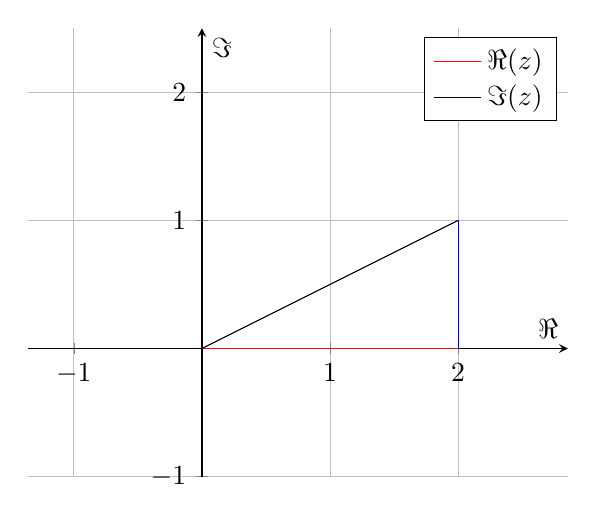
\begin{tikzpicture}
	\begin{axis}[
		axis lines = middle,
		axis equal,
		grid=both,
		xlabel=\(\Re\),
		ylabel=\(\Im\),
		xmin=-1,
		xmax=2.5,
		ymin=-1,
		ymax=2.5
		]
		\addplot[mark=none, red, samples=2, domain=(0:2)] {0};
		\addlegendentry{$\Re(z)$};
		\draw[blue] (2,0) -- (2,1);
		\addlegendentry{$\Im(z)$};
		\addplot[domain=(0:2)] {0.5 * x};
		\end{axis}
\end{tikzpicture}
\end{center}
$\Re$ and $\Im$ specify which part of the complex number is used. For example, with $z=2+\iu$, the real portion of the complex number would be 2, and the imaginary portion of the complex number would be 1, as there is 1 imaginary unit in $z$.\\
It is also important to consider when a $z$ is purely \textsl{imaginary} or purely \textsl{real}.
\begin{tcolorbox}[
		floatplacement=t,
		float,
		colframe = keyIdea,
		title= $\Re$ and $\Im$]
		{
			Consider a function, $z$ that has two components: a \textsl{real} component, and its \textsl{imaginary} component. The $\Re$ and $\Im$ give values that correspond with the real or imaginary portion of the function respectively.\\
			\hspace{1.3em}
			\begin{center}
				$z= a+b\hspace{0.2em}\iu$\\
				\color{purple}{$\therefore \Re(z) = a$; $\Im(z)= b$}
			\end{center}
		}
	\end{tcolorbox}
Now, before you spend 20 minutes trying to write a fancy $\Re$ or $\Im$ on your exams, it is possible to write ``Re(z)" and ``Im(z)" as is and still convey the same meaning. As seen with the previous figure, the components of complex  numbers were $\Re(z)$ and $\Im(z)$. It is imperative to understand complex numbers as a set of coordinates that can be separated while problem solving.
\section{Euler's Form}
{\color{red}{\Large{This topic will only make sense after going through the Trigonometry section.}}}
As you may recall a unit circle is defined as $x^2 + y^2 = 1$. 
\end{document}
